
\chapter{Thinking like an economist}

Every field of study has its own language and its own way of thinking.
The most important is to learn the economist's of thinking.


\section{The economist as scientist}

Economist try to address their subject with a scientist's objectivity:
\begin{itemize}
\item devise theories
\item collect data
\item analyze these data in an attempt to verify or refute their theories
\end{itemize}

\begin{tcolorbox}
  The essence of science is the scientific method -- the dispassinate development and testing of theories about how the world works.
\end{tcolorbox}

As Albert Einstein once put it, ``The whole of science is nothing more than the refinement of everyday thinking''.


\subsection{The scientific method}

The scientific method:
\begin{enumerate}
\item observation
\item theory
\item more observation
\end{enumerate}

Although economists use theory and observation like other scientists, they do face an obstacle that makes their task especially challenging: Experiments are often difficult in economics.

\subsection{The role of assumptions}

Assumptions can make the world easier to understand.
The art in scientific thinking is deciding which assumptions to make.
Economists use different assumptions when studying the short-run and long-run efects of a change in the quantity of money.

\subsection{Economic models}

Economists use models that are most often composed of diagrams and equations to learn about the world.
Economic models omit many details to allow us to see what is truely important.
An economist's model does not include every feature of the economy.
All models are built with assumptions.
Economists assume away many of the details of the economy that are errelevant for studying the question at hand.
All models simplify reality in order to improve our understanding of it.

\subsection{The circular-flow diagram}

Circular-flow diagram: a visual model of the economy that shows how dollars flow through markets among households and firms.


\begin{figure}[!ht]
  \centering
  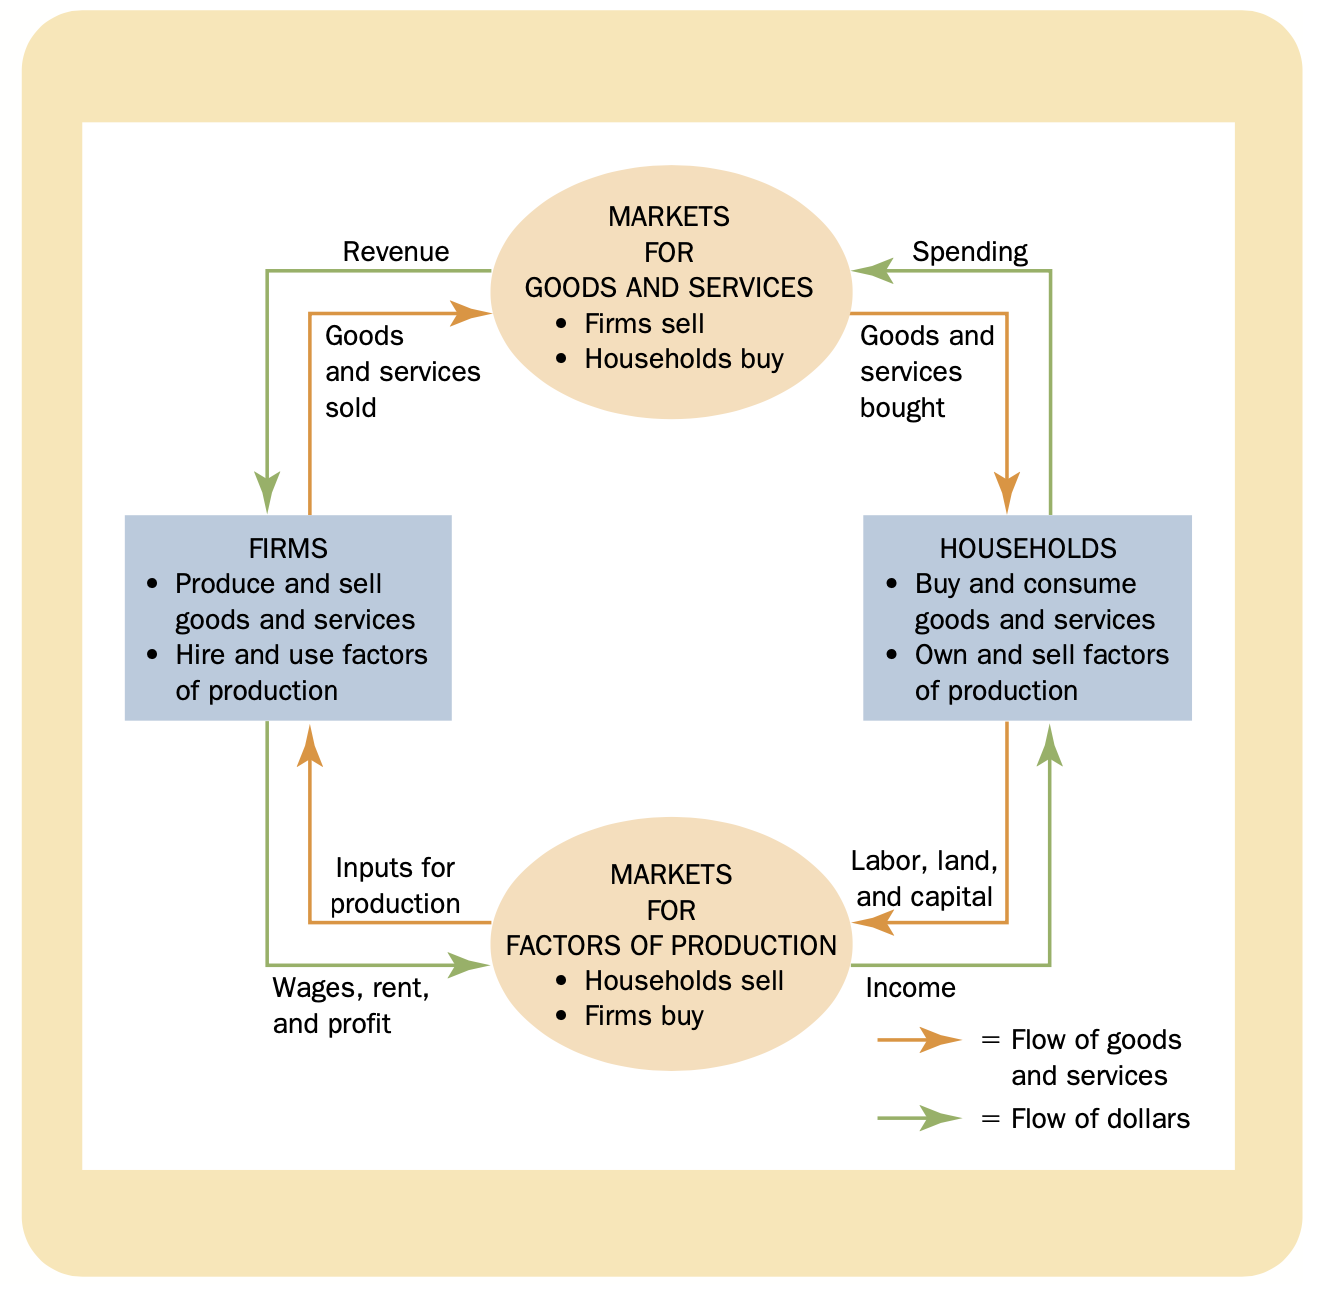
\includegraphics[width=\textwidth]{pics/circular-flow.png}
  \caption{The circular flow}
  \label{fig:circular-flow}
\end{figure}


\subsection{The production possibilities frontier}

Most economics models are built using the tools of mathematics.
Here we consider one of the simplest such models, called the production possibilities frontier.
The \keyword{production possibilities frontier} is a graph that shows the various combinations of output that the economy can possibly produce given the available factors of production and the available production technology that firms can use to turn these factors into output. The graph is shown in Figure \ref{fig:the-production-possibilities-frontier}.



\begin{figure}[!ht]
  \centering
  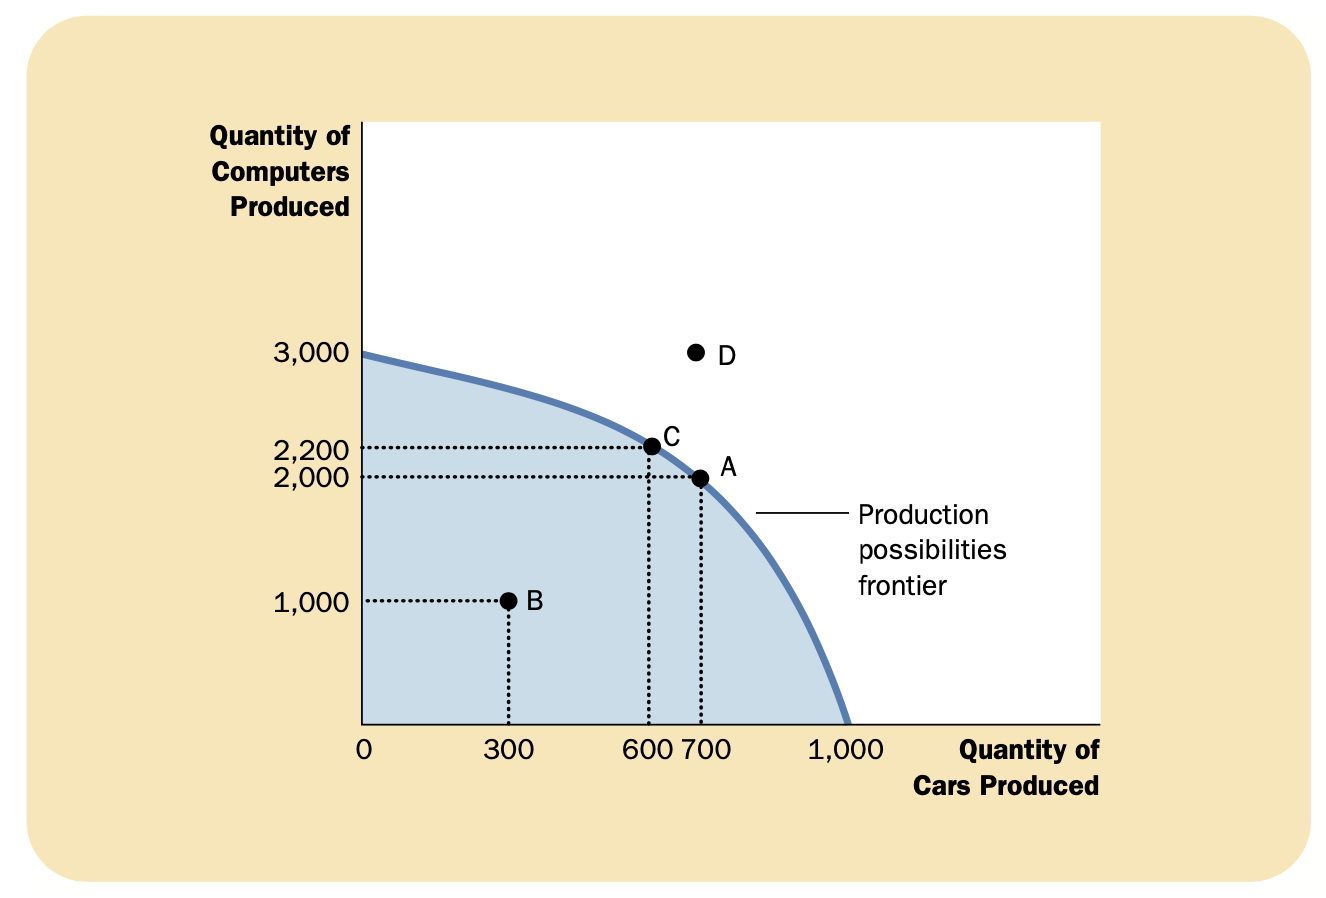
\includegraphics[width=\textwidth]{pics/the-production-possibilities-frontier}
  \caption{The production possibilities frontier}
  \label{fig:the-production-possibilities-frontier}
\end{figure}



An outcome is said to be \keyword{efficient} if the economy is getting all it can from the scarce resources it has available.
Points on (rather than inside) the production possibilities frontier represent efficient levels of production.



\subsection{Microeconomics and macroeconomics}

The field of economics is traditionally divided into two broad subfields.
\keyword{Microeconomics} is the study of how households and firms make decisions and how they interact in specific markets.
\keyword{Macroeconomics} is the study of economywide phenomena.



Microeconomics and macroeconomics are closely intertwined.
Because changes in the overall economy arise from the decisions of millions of individuals, it is impossible to understand macroeconomic developments without considering the associated microeconomic decisions.
Despite the inherent link between microeconomics and macroeconomics, the two fields are distinct.


\section{The economist as policy adviser}


When economists are trying to explain the world, they are \keyword{scientists}.
When they are trying to help improve it, they are \keyword{policy advisers}.


\subsection{Positive versus normative analysis}


Because scientists and policy advisers have different goals, they use language in different ways.
In general, statements about the world are of two types.
One type is positive.
\keyword{Positive statements} are descriptive.
They make a clain about how the world \keyword{is}.
A second type of statement is normative.
\keyword{Normative statements} are are prescrptive.
They make a clain about how the world \keyword{ought to be}.


A key difference between positive and normative statements is how we judge their validity.
We can, in principle, confirm or refute positive statements by exam- ining evidence.
By contrast, evaluating normative statements involves values as well as facts.


Much of economics just tries to explain how the economy works.
Yet often the goal of economics is to improve how the economy works.
When you hear economists making normative statements, you know they have crossed the line from scientist to policy adviser.



\section{Why economists disagree}

Why do economists so often appear to give conflicting advice to policymakers?
There are two basic reasons:
\begin{itemize}
\item Economists may disagree about the validity of alternative positive theories about how the world works.
\item Economists may have different values and, therefore, different normative views about what policy should try to accomplish.
\end{itemize}


Because of differences in scientific judgments and differences in values, some disagreement among economists is inevitable.
Yet one should not overstate the amount of disagreement.
In many cases, economists do offer a united view.


You might find it helpful to keep in mind some advice from the great economist John Maynard Keynes:

\begin{tcolorbox}
The study of economics does not seem to require any specialized gifts of an unusually high order. Is it not \dots a very easy subject compared with the higher branches of philosophy or pure science? An easy subject, at which very few excel! The paradox finds its explanation, perhaps, in that the master-economist must possess a rare combination of gifts. He must be mathematician, historian, statesman, philosopher—in some degree. He must understand symbols and speak in words. He must contemplate the particular in terms of the general, and touch abstract and concrete in the same flight of thought. He must study the present in the light of the past for the purposes of the future. No part of man’s nature or his institutions must lie entirely outside his regard. He must be purposeful and disinterested in a simultaneous mood; as aloof and incorruptible as an artist, yet sometimes as near the earth as a politician.
\end{tcolorbox}

